\documentclass[12pt]{article}
\usepackage{hyperref}
\usepackage[warn]{mathtext}
\usepackage[T2A]{fontenc}
\usepackage[utf8]{inputenc}
\usepackage[russian]{babel}
\usepackage{cite}
\usepackage{amsfonts}
\usepackage{lineno}
\usepackage{subfig}
\usepackage{graphicx}
\usepackage{xcolor}
\usepackage{bm}
\usepackage{graphicx}
\usepackage{amssymb}
\usepackage{hyperref}
\usepackage[left=2cm,right=2cm,top=2cm,bottom=2cm]{geometry}
\usepackage{indentfirst}
\DeclareSymbolFont{T2Aletters}{T2A}{cmr}{m}{it}

\DeclareGraphicsExtensions{.png,.jpg,.svg,.pdf}
\author{Карцев Вадим}
%\date{7 октября 2021 г.}
\title{Лабораторная работа 8.1

Тепловое излучение}

\begin{document}

  \maketitle

  \textbf{Цель работы:} измерение температуры модели АЧТ с помощью пирометра и
  термопары, исследование излучения накаленных тел, подтверждение закона
  Стефана-Больцмана и определение постоянных Стефана-Больцмана и Планка.

  \vspace{0.3cm}

  \textbf{В работе используются:} Оптический пирометр, модель АЧТ, керамическая
  трубка с кольцами, вольфрамовая лампа, неоновая лампа, блок питания, цифровые
  вольтметры.

  \section*{Аннотация}

    В ходе работы были измерены температуры АЧТ и серых тел, подтвержден закон
    Стефана-Больцмана, а также определены постоянные Стефана-Больцмана
    ($\sigma = 5.549 \cdot 10^{-8} \frac{Вт}{м^2 \cdot К^2}$) и Планка
    ($h = 6.667 \cdot 10^{-34} Дж \cdot с$), в полной мере совпавшие с
    теоретическими значениями.

  \tableofcontents

  \newpage
  \section{Теоретическая справка}

    Для того, чтобы измерить температуру тела без непосрадственного контакта,
    используют метод оптической пирометрии. Он основан на определении температуры
    испускаемого излучения, на основе которой можно сделать вывод о
    термодинамической температуре тела.

    Различают три температуры, функционально связанные с истинной
    термодинамической температурой и излучательной способностью тела:
    радиационную $T_{рад}$, цветовую $T_{цв}$ и яркостную $T_{яр}$.

    В работе измеряется яркостная температура. \textbf{Яркостная температура} -
    это температура абсолютно чёрного тела, при которой его спектральная
    испускательная способность равна спектральной испускательной способности
    исследуемого тела при той же длине волны.

    Яркостная температура серого тела всегда ниже его термодинамической температуры.
    Это связано с тем, что любое серое тело излучает меньше, чем АЧТ при той
    же температуре. Зависимость между яркостной и термодинамической
    температурами вольфрама приведена на рисунке \ref{fig:volfram}.

    \begin{figure}[h]
        \centering
        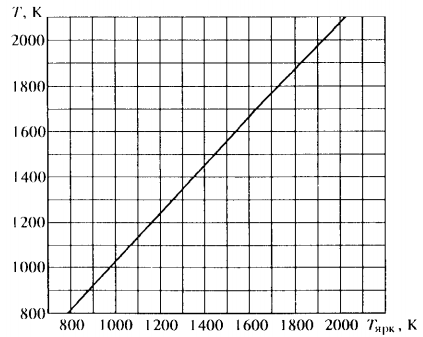
\includegraphics[width=10cm]{fig2.png}
        \caption{График зависимости $T = f(T_{b_r})$ для вольфрама}
        \label{fig:volfram}
    \end{figure}

    По результатам измерений мощности излучения вольфрамовой нити можно судить
    о справедливости закона Стефана-Больцмана. Если бы нить излучала как АЧТ, то
    баланс потребляемой и излучаемой энергии определялся бы соотношением

    \begin{equation} \label{eq:en1}
        W = \sigma S (T^4 - T_0^4),
    \end{equation}

    где $W$ - потребляемая нитью электрическая мощность, $S$ - площадь
    излучающей поверхности нити, $T$ - температура нити, $T_0$ - температура
    окружающей среды. Вольфрамовая нить излучает как серое тело, и ее излучение
    ослаблено по сравнению с АЧТ в $\varepsilon_T$ раз для любой длины
    волны при температуре тела Т. Предположим, что нить излучает
    как серое тело и $T_0 \ll T$. Тогда выражение
    \ref{eq:en1} можно переписать в виде

    \begin{equation} \label{eq:en2}
        W = \varepsilon_T S \sigma T^4
    \end{equation}

    В справедливости закона Стефана-Больцмана можно убедиться, построив график
    зависимости $\ln W(\ln T)$. По углу наклона прямой аппроксимации можно
    определить показатель степени $n$ исследуемой зависимости. В пределах
    погрешности показатель степени должен быть близок к четырём.

    Также из формулы \ref{eq:en2} можно определить постоянную Стефана-Больцмана.

  \section{Описание экспериментальной установки}

    \begin{figure}[h]
      \begin{minipage}[h]{0.49\linewidth}
        \center{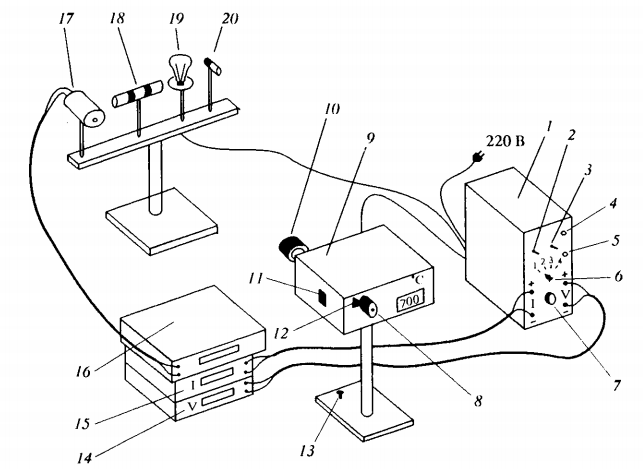
\includegraphics[width=\linewidth]{fig1.png}}
        \caption{Схема экспериментальной установки}
      \end{minipage}
      \begin{minipage}[h]{0.49\linewidth}
        1 - блок питания;
        2 - тумблер включения питания образцов;
        3 - тумблер нагрева нити пирометра;
        4 - кнопка "Нагрев нити";
        5 - кнопка "охлаждение нити";
        6 - тумблер переключения образцов;
        7 - регулятор мощности нагрева образцов;
        8 - окуляр пирометра;
        9 - корпус пирометра;
        10 - объектив пирометра;
        11 - переключение диапазонов;
        12 - ручка смещения красного светофильтра;
        13 - регулировочный винт;
        14 - вольтметр (напряжение на лампе накаливания);
        15 - амперметр (ток через образцы);
        16 - вольтметр в цепи термопары;
        17 - модель АЧТ;
        18 - трубка с кольцами из материалов с различной излучательной
        способностью;
        19 - лампа накаливания;
        20 - неоновая лампочка
      \end{minipage}
      \label{fig:setup}
    \end{figure}

    Исследуемые в работе образцы:
    \begin{itemize}
        \item \textbf{Модель абсолютно чёрного тела} - керамическая трубка,
        закрытая с одного конца и окружённая для теплоизоляции внешним кожухом.
        Температура в трубке измеряется с помощью термопары хромель-алюмель
        \item \textbf{Керамическая трубка с набором колец}, нагреваемая изнутри
        нихромовой спиралью.
        \item \textbf{Вольфрамовая нить электрической лампочки}
        \item \textbf{Неоновая лампочка}
    \end{itemize}

  \newpage
  \section{Ход работы}

    \subsection{Изучение работы оптического пирометра}

      Измерим температуру модели АЧТ с помощью оптического пирометра. Для этого
      направим окуляр на АЧТ, установим красный светофильтр и будем менять
      температуру нити пирометра до тех пора, пока она не будет сливаться с
      накаленным АЧТ. Проведем 4 измерения и проверим, насколько точны
      полученные с помощью пирометра значения.\\

      \begin{tabular}{ || c || c | c | c | c || }
        \hline
        Температура на пирометре & $915$ & $915$ & $932$ & $926$ \\ \hline
        Напряжение на термопаре & $36.8$ & $36.8$ & $36.9$ & $37.1$ \\ \hline
        Температура АЧТ & $897.56$ & $897.56$ & $900.00$ & $904.88$ \\ \hline
        Разница значений & $1.92 \%$ & $1.92 \%$ & $3.49 \%$ & $2.31 \%$ \\
        \hline
      \end{tabular}\\

      Легко заметить, что значения, полученные с помощью пирометра, достаточно
      близки со значениями, измеренными с помощью термопары и отличаются
      максимум на $3.49 \%$.

    \subsection{Измерение яркостной температуры тел}

      Раскалив керамическую трубку до свечения, измерим ее температуру с
      помощью пирометра.

      Для керамической трубки получим значения в районе
      $760 - 770 \hspace{0.2cm} ^{\circ}C$ на разных частях трубки.

      Для колец точно распознать температуру оказалось практически невозможно,
      так как значения выходили за нижнюю границу возможностей пирометра. Так,
      температуры колец приблизительно находились в рамках
      $740 - 750 \hspace{0.2cm} ^{\circ}C$

    \subsection{Проверка закона Стефана-Больцмана}

      Будем выставлять температуру нити пирометра с шагом
      $100 \hspace{0.1cm} ^{\circ}C$. Мощность лампы будем регулировать до
      совпадения с температурой нити пирометра. Составим таблицу соответствия
      тока и напряжения, подаваемых на лампу с термодинамической температурой.
      Термодинамическую температуру получим с помощью
      \hyperref[fig:volfram]{графика зависимости} термодинамической температуры
      от яркостной температуры для вольфрама.\\

      \begin{tabular}{ || c || c | c | c | c | c | c | c | c | c | c | c || }
        \hline
        $I$, $мА$ & $0.683$ & $0.75$ & $0.81$ & $0.86$ & $0.9$ & $0.96$ & $1.05$ & $1.14$ & $1.23$ & $1.28$ & $1.36$ \\ \hline
        $U$, $В$ & $21.1$ & $26.3$ & $31.9$ & $36.6$ & $40$ & $47$ & $54.9$ & $63.9$ & $73.1$ & $78.7$ & $88.9$ \\ \hline
        $T_{ярк}$, $^{\circ}C$ & $900$ & $1000$ & $1100$ & $1200$ & $1300$ & $1400$ & $1500$ & $1600$ & $1700$ & $1800$ & $1900$ \\ \hline
        $T$, $^{\circ}C$ & $936$ & $1040$ & $1144$ & $1248$ & $1352$ & $1456$ & $1560$ & $1664$ & $1768$ & $1872$ & $1976$ \\
        \hline
      \end{tabular}\\

      \subsubsection{Определение порядка зависимости}

        Для определения порядка зависимости в проведенном эксперименте,
        прологарифмируем выражение вида

        $$
          y = \alpha x^{\beta} \Rightarrow
          \ln y = \ln \left(\alpha x^{\beta}\right) =
          \ln \alpha + \ln \left(x^{\beta}\right) =
          \ln \alpha + \beta \ln x
        $$

        Таким образом, можно получить степень зависимости, построив график
        зависимости в логарифмическом масштабе. Построим этот график.

        \newpage
        \begin{figure}[h]
            \centering
            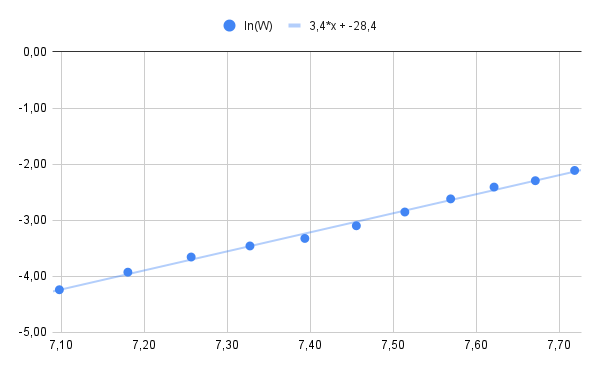
\includegraphics[width=0.7\linewidth]{st-bm.png}
            \caption{Зависимость}
            \label{fig:plot}
        \end{figure}

        Таким образом, экспериментально мы получили зависимость $3.4 \approx 3$
        степени.

      \subsubsection{Определение постоянной Стефана-Больцмана}

        Определим постоянную Стефана-Больцмана при температуре
        $1872 \hspace{0.1cm} ^{\circ} C$. Примем $\varepsilon_T \approx 0.232$,
        $S = 0.36$ $см^2$

        $$
          \sigma = \frac{W}{\varepsilon_T S T^4} =
          \frac{1.28 \cdot 10^{-3} \cdot 78.7}
          {0.232 \cdot 0.36 \cdot 10^{-4} \cdot (1872 + 273.15)^4} \approx
          9.8 \cdot 10^{-10} \frac{Вт}{м^2 \cdot К^2}
        $$

        Так же можно вычислить постоянную Стефана-Больцмана можно вычислить из
        построенного логарифического графика.

        $$
          \ln \left(\sigma \varepsilon_T S\right) = -28.4
        $$

        $$
          \sigma = \frac{e^{-28.4}}{\varepsilon_T S} \approx 5.549 \cdot 10^{-8}
          \frac{Вт}{м^2 \cdot К^2}
        $$

        Различия в значениях постоянной Стефана-Больцмана обусловлены тем, что в
        первом случае мы считаем зависимость теоретической (степень при $T$
        $n = 4$)

      \subsubsection{Определение постоянной Планка}

        Рассчитаем так же значение постоянной Планка

        $$
          \sqrt[3]{\frac{2 \pi^5 k_Б^4}{15 c^2 \sigma}} \approx
          6.667 \cdot 10^{-34} Дж \cdot с
        $$

    \subsection{Измерение яркостной температуры неоновой лампочки}

      С помощью пирометра определим яркостную температуру неоновой лампочки.
      Она оказалась равна $846 \hspace{0.1cm} ^{\circ} C$. Полученное значение
      очень сильно разнится с термодинамической температурой лампочки. Ее
      температура примерно совпадает с комнатной температурой.

      Данное явление объясняется отличием принципа действия неоновой лампочки,
      которая не является абсолютно черным или серым телом. Ее излучение
      возникает засчет перехода электронов между уровнями.

  \section{Вывод}

    В ходе выполнения работы было изучено тепловое излучение модели АЧТ и
    моделей серых тел (керамической трубки, колец и вольфрамовой нити), а так же
    неоновой лампы. Отличия для различных моделей серых тел обусловлены тем, что
    они имеют разные коэффициенты ослабления по сравнению с АЧТ.

    Была выяснена ошибка в измерении температур с помощью оптического пирометра,
    которая не превышала $3.49 \%$.

    Так же был подтвержден закон Стефана-Больцмана ($W \propto T^4$). В ходе
    эксперимента был получен фактический коэффициент $3.4$, что достаточно
    близко к действительному значени. Отличия обусловлены слудующими факторами:

    \begin{itemize}
      \item Ошибка в показаниях пирометра
      \item Ошибка визуальных наблюдений через пирометр
      \item Значительный теплоотвод от нити
      \item Потери на остальных частях цепи, которые привели к неверному
      определению мощности лампы
    \end{itemize}

    Так же были определены постоянная Стефана-Больцмана (двумя способами) и
    постоянная Планка. Второй способ определения постоянной Стефана-Больцмана
    оказался более точен, так как базируется на реальной зависимости с учетом
    всех потерь и неточностей.\\

    \begin{tabular}{ || c || c | c | }
      \hline
       & Экспериментальное значение & Теоретическое значение \\ \hline\hline
       $\sigma$, $\frac{Вт}{м^2 \cdot К^2}$ & $5.549 \cdot 10^{-8}$ & $5.67 \cdot 10^{-8}$ \\ \hline
       $h$, $Дж \cdot с$ & $6.667 \cdot 10^{-34}$ & $6.62 \cdot 10^{-34}$ \\ \hline
    \end{tabular}\\

    Как можно заметить, экспериментальные данные совпадают с теоретическими в
    достаточной мере.

    Кроме того, в ходе работы было выяснено, что для неоновой лампочки яркостная
    температура не соответствует термодинамической, так как она не является
    моделью АЧТ или серого тела.

\end{document}
